\section{Theoretical Analysis}
\label{sec:analysis}

In this section, the circuit shown in Figure~\ref{fig:circuitol1} is analysed
theoretically using methods: Node and Mesh Analysis.

\subsection{Node Analysis}
\label{subsec:node_analysis}

Before applying the method, it is important to discuss how it works.\\
In general, it consists of discovering the voltages associated with each node of the circuit - they are the unknown variables in our equations. \\
In order to obtain these relations, one has to apply \textit{Kirchhoff}'s Current Law (KCL) to the nodes, always having in mind that nodes on the ends of branches containing Independent Voltage Sources cannot be analysed in this way. \\

\[
\begin{bmatrix}
1 & 0 & 0 & 0 & 0 & 0 & 0 \\
0 & 0 & 0  & 1 & 0 & K_c*G_6 & -1 \\
G_1 & -(G_1+G_2+G_3) & G_2 & G_3 & 0 & 0 & 0  \\
0 & K_b+G_2 & -G_2 & -K_b & 0 & 0 & 0 \\
0 & G_2 & -G_2 & G_5 & -G_5 & 0 & 0 \\
0 & 0 & 0 & 0 & 0 & G_6+G_7 & G_7 \\
0 & G_3 & 0 & -(G_3+G_4+G_5) & G_5 & G_7 & -G_7
\end{bmatrix}
\begin{bmatrix}
V_1 \\
V_2 \\
V_3 \\
V_4 \\
V_5 \\
V_6 \\
V_7 
\end{bmatrix}
=
\begin{bmatrix}
V_a \\
0 \\
0 \\
0 \\ 
-I_d \\
0 \\
I_d 
\end{bmatrix}
\] \relax


\subsection{Mesh Analysis}
\label{subsec:mesh_analysis}

In this case 
Usually, we create \textit{fictious} currents in each mesh and we then apply \textit{Kirchhoff}'s Voltage Law (KVL) to either meshes or loops, depending on if it

\[
\begin{bmatrix}
R_1+R_3+R_4 & R_3 & R_4 \\
-K_bR_3 & 1-K_bR_3 & 0 \\
R_4 & 0 & (R_4+R_6+R_7-K_c)
\end{bmatrix}
\begin{bmatrix}
I_1 \\
I_2 \\
I_3
\end{bmatrix}
=
\begin{bmatrix}
V_a \\
0 \\
0
\end{bmatrix}
\]

\section{Time response}

The circuit consists of a single V-R-C loop where a current $i(t)$ circulates. The
voltage source $v_I(t)$ drives its input, and the output voltage $v_O(t)$ is taken from
the capacitor terminals. Applying the Kirchhoff Voltage Law (KVL), a single
equation for the single loop in the circuit can be written as

\begin{equation}
  Ri(t) + v_O(t) = v_I(t).
  \label{eq:kvl}
\end{equation}

Because $v_O$ is the voltage between capacitor C's plates, it is related to the
current $i$ by
\begin{equation}
  i(t) = C\frac{dv_O}{dt}.
\end{equation}

Hence, Equation~(\ref{eq:kvl}) can be rewritten as
\begin{equation}
  RC\frac{dv_O}{dt} + v_O(t) = v_I.
  \label{eq:kvl2}
\end{equation}

Equation~(\ref{eq:kvl2}) is a linear differencial equation whose solution is a
superposition of a natural solution $v_{On}$ and a forced solution $v_{Of}$:

\begin{equation}
  v_O(t) = v_{On}(t) + v_{Of}(t).
  \label{eq:vo_sol}
\end{equation}

As learned in the theory classes the natural solution is of the form
\begin{equation}
  v_{On}(t) = Ae^{-\frac{t}{RC}},
  \label{eq:vo_nat}
\end{equation}
where $A$ is an integration constant.

The forced solution is of the form given in Equation~(\ref{eq:vo_for}) and is
illustrated in Figure~\ref{fig:forced}.

\begin{equation}
  V_{Of}(t) = |\bar{V}_{Of}| cos(\omega t + \angle \bar{V}_{Of}),
  \label{eq:vo_for}
\end{equation}

\lipsum[1-1]


%\begin{figure}[h] \centering
%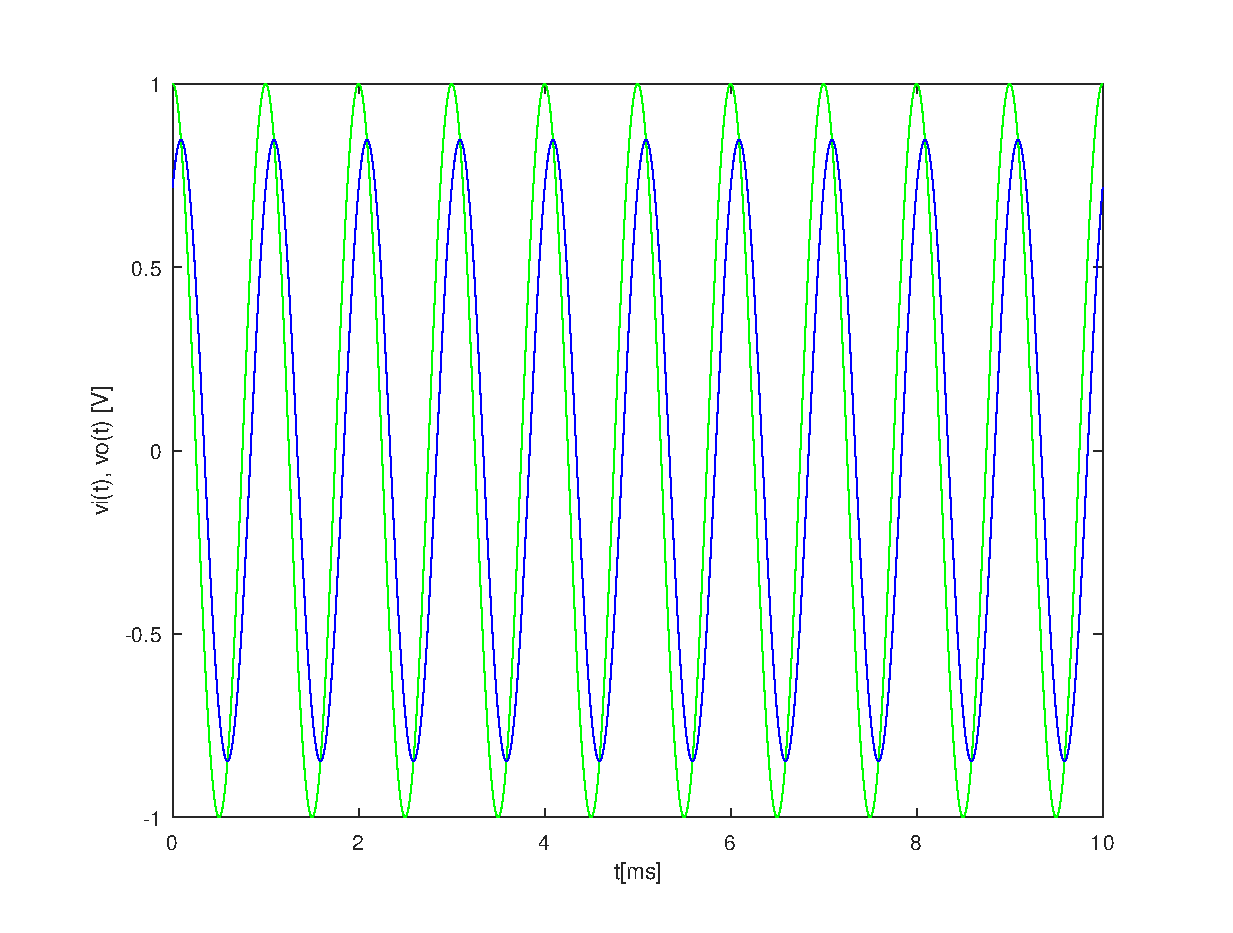
\includegraphics[width=0.8\linewidth]{forced.eps}
%\caption{Forced sinusoidal response.}
%\label{fig:forced}
%\end{figure}

\section{Frequency response}

\lipsum[1-1]


